\section{Diseño del sistema}

En la figura~\ref{fig:chapter_1.overview} vimos un esquema general del sistema, el cual recibe documentos en formato
PDF y genera objetos que contienen la información más importante de los mismos.
En la figura~\ref{fig:chapter_1.specific_b} vimos que se va a incluir también el desarollo de dos interfaces, una web
y una de línea de comandos.

En la figura~\ref{fig:chapter_4.overview} vemos que el sistema tiene dos componentes principales: el \textit{Reader}
y el \textit{Generator}

\begin{figure}[ht]
    \begin{center}
        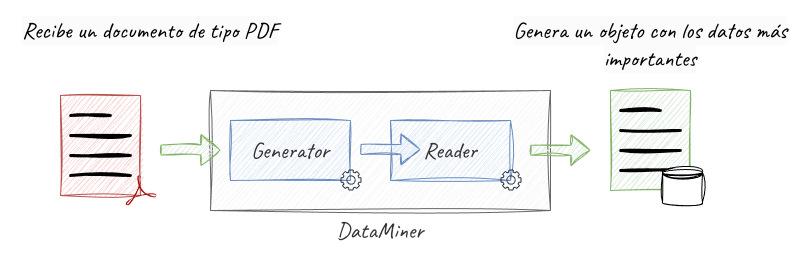
\includegraphics[width=\textwidth]{./chapter/4/images/chapter_4.overview}
        \caption{Esquema de los componentes principales}
        \label{fig:chapter_4.overview}
    \end{center}
\end{figure}

\subsection*{Componente \textit{Generator}}

Este componente sirve como el motor inicial en el proceso, encargado de convertir documentos de cualquier formato a
texto plano.

Se compone de tres conjuntos de elementos y un orquestador al que llamaremos \textit{Engine} responsable de la
coordinación de las operaciones.

Diagrama UML del componente generator.

\subsubsection*{Preprocesadores}
Los preprocesadores preparan el documento original para facilitar su conversión a texto.
En esta implementación no se ha desarrollado ningún preprocesador.

Comunicación del Engine con los preprocesadores definidos.


\subsubsection*{Procesadores}
Actúan como el núcleo del Generator, donde se realiza la conversión efectiva del documento a texto. Funcionan mediante
un sistema competitivo donde varios procesadores evalúan su propia aptitud para manejar el documento en cuestión,
seleccionando el más adecuado para llevar a cabo la tarea.

Este enfoque modular y competitivo asegura que el procesamiento del texto sea no solo eficiente, sino también
extremadamente flexible, adaptándose a las variaciones en la naturaleza de los documentos procesados.


Comunicación del Engine con los procesadores definidos.

En la actual implementación, hemos desarrollado un único procesador especializado en transformar documentos PDF a
texto. Este procesador utiliza la utilidad de línea de comandos `pdftotext` para llevar a cabo la conversión (Glyph \&
Cog, 2023).

\subsubsection*{Postprocesadores}
Estos componentes perfeccionan el texto generado, eliminando errores como caracteres no UTF-8 y espacios en blanco
innecesarios, lo que mejora significativamente la calidad del texto resultante. En esta implementación, se han
desarrollado varios post-procesadores:

\begin{itemize}
    \item
    Word Limit PostProcessor: Se detectó que los elementos de interés, como nombres, documentos de identidad y fechas de
    contratos, típicamente aparecen en las primeras páginas. Este procesador limita el análisis a las primeras N
    palabras del documento.
    \item UTF8 PostProcessor: Implementado tras detectar caracteres no UTF-8 en algunos documentos, este post-procesador
    elimina dichos caracteres.
    \item Character Replace PostProcessor: Desarrollado para eliminar caracteres específicos que complicaba las pruebas.
\end{itemize}

\subsubsection*{Engine}
Este es el orquestador del componente, encargado de hacer las llamadas a los demás elementos registrados en la
aplicación. Coordina el flujo entre los pre-procesadores, procesadores y post-procesadores para asegurar que el
documento sea procesado de manera correcta.

\subsection*{Reader}
El componente Reader juega un papel crucial en el proceso de interpretación y procesamiento del texto plano obtenido a
partir de la salida del componente Generator anterior..

Funciona mediante un sistema de procesadores organizados en una única capa, que opera bajo un mecanismo competitivo
similar al del componente Generator. En este sistema, los procesadores compiten entre sí para determinar cuál es el más
adecuado para analizar y extraer la información estructurada necesaria del texto.

Diagrama UML del componente Reader.

\subsubsection*{Procesadores}
Cada uno de estos procesadores es invocado secuencialmente para evaluar su idoneidad en el manejo del documento
específico..

Una vez seleccionado, el procesador elegido procede a ejecutar una serie de tareas que incluyen la identificación y
extracción de entidades clave. En esta implementación, se han desarrollado los siguientes procesadores:

\begin{itemize}
    \item Residential Lease Processor: Evalúa si el documento se trata de un contrato de alquiler de vivienda entre
    particulares. En caso afirmativo, extrae la información más relevante del mismo, como los nombres de los
    arrendadores, los arrendatarios y la fecha del contrato.
    \item Vehicle Sale And Purchase Processor: Evalúa si el documento se trata de un contrato de compraventa de
    vehículos
    entre particulares. En caso afirmativo, extrae la información más relevante del mismo, como los nombres de los
    compradores y vendedores y la fecha de la transacción.
\end{itemize}

\subsubsection*{Engine}
Este es el orquestador del componente, encargado de hacer las llamadas a los demás elementos registrados en la
aplicación, en este caso únicamente los procesadores.

